\subsection{Software Privilege Levels}
\label{sec:rings}

% Outcome: enumerate all software actors and their trust relationships

In an Infrastructure-as-a-Service (IaaS) cloud environment, such as Amazon EC2,
commodity CPUs run software at four different privilege levels, shown in
Figure~\ref{fig:cpu_rings}.

\begin{figure}[hbtp]
  \centering
  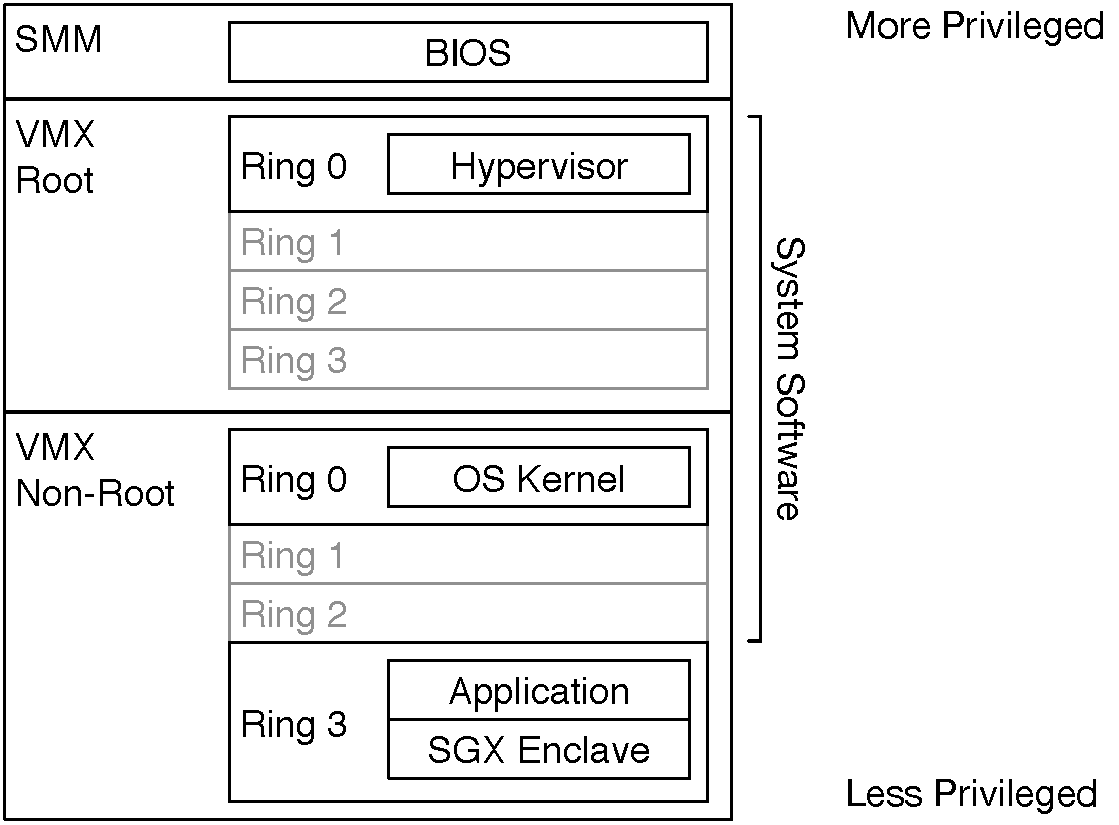
\includegraphics[width=85mm]{figures/cpu_rings.pdf}
  \caption{
    The privilege levels in the x86 architecture, and the software that
    typically runs at each security level.
  }
  \label{fig:cpu_rings}
\end{figure}

Each privilege level is strictly more powerful than the ones below it, so a
piece of software can freely read and modify the code and data running at less
privileged levels. Therefore, a software module can be compromised by any piece
of software running at a higher privilege level. It follows that a software
module implicitly trusts all the software running at more privileged levels,
and a system's security analysis must take into account the software at all
privilege levels.

% System Management Mode: SDM S 34

\textit{System Management Mode} (SMM) is intended for use by the motherboard
manufacturers to implement features such as fan control and deep sleep, and/or
to emulate missing hardware. Therefore, the bootstrapping software
(\S~\ref{sec:booting}) in the computer's firmware is responsible for setting up
a continuous subset of DRAM as \textit{System Management RAM}~(SMRAM), and for
loading all the code that needs to run in SMM mode into SMRAM. The SMRAM
enjoys special hardware protections that prevent less privileged software from
accessing the SMM code.

IaaS cloud providers allow their customers to run their operating system of
choice in a virtualized environment. Hardware
virtualization~\cite{uhlig2005vmx}, called \textit{Virtual Machine Extensions}
(VMX) by Intel, adds support for a \textit{hypervisor}, also called a
\textit{Virtual Machine Monitor} (VMM) in the Intel documentation. The
hypervisor runs at a higher privilege level (VMX root mode) than the operating
system, and is responsible for allocating hardware resources across multiple
operating systems that share the same physical machine. The hypervisor uses the
CPU's hardware virtualization features to make each operating system believe it
is running in its own computer, called a \textit{virtual machine} (VM).
Hypervisor code generally runs at ring 0 in VMX root mode.

Hypervisors that run in VMX root mode and take advantage of hardware
virtualization generally have better performance and a smaller codebase than
hypervisors based on binary translation \cite{rosenblum2005virtualization}.

The systems research literature recommends breaking up an operating system into
a small \textit{kernel}, which runs at a high privilege level, known as the
\textit{kernel mode} or \textit{supervisor mode} and, in the Intel
architecture, as \textit{ring 0}. The kernel allocates the computer's resources
to the other system components, such as device drivers and services, which run
at lower privilege levels. However, for performance reasons\footnote{Calling a
procedure in a different ring is much slower than calling code at the same
privilege level.}, mainstream operating systems have large amounts of code
running at ring 0. Their \textit{monolithic kernels} include device drivers,
filesystem code, networking stacks, and video rendering functionality.

Application code, such as a Web server or a game client, runs at the lowest
privilege level, referred to as \textit{user mode} (\textit{ring 3} in the
Intel architecture). In IaaS cloud environments, the virtual machine images
provided by customers run in VMX non-root mode, so the kernel runs in VMX
non-root ring 0, and the application code runs in VMX non-root ring 3.
